%!TEX root = master.tex

\section{Policy gradient methods}
Policy gradient methods are a class of model-free reinforcement learning algorithms that directly optimizes the policy, maps the states to action by using gradient descent. By using gradient of the expected return with respect to the policy parameters, these class of methods iteratively updates the policy to improve the performance. 

\subsection*{Value-based vs Policy based RL}
The value-based RL methods are what we have looked at so far. Here we learn the value function and act greedily ($\epsilon$-greedy). In policy-based methods we don't use a value function, but learn a policy instead. In the next chapters we will take a look at Actor-critic methods were we learn the value function and policy.

\begin{figure}[ht!]
\centering
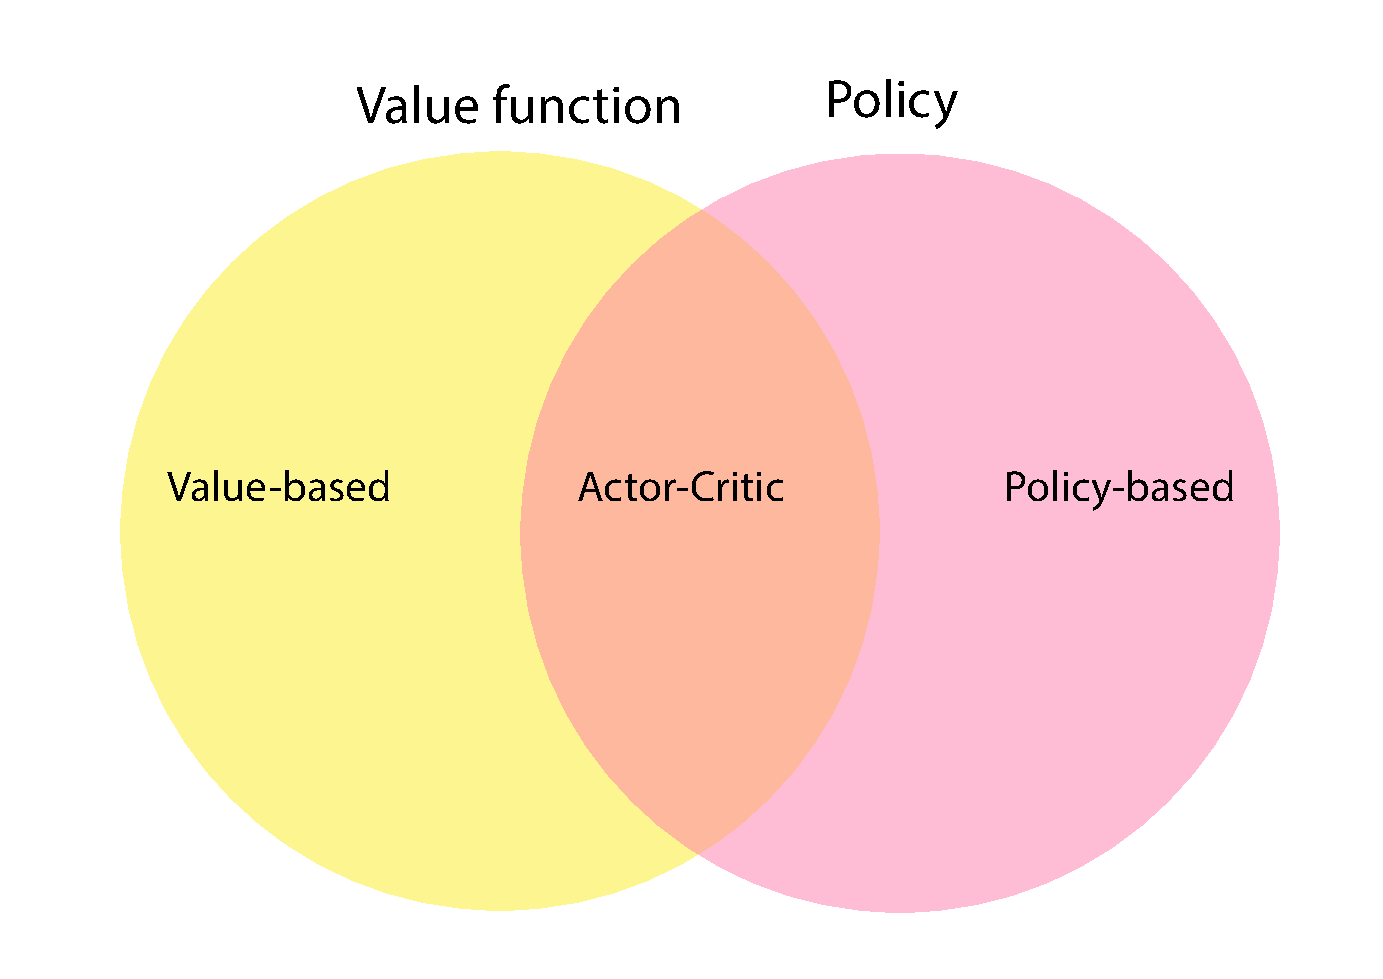
\includegraphics[width=80mm]{figures/valuepolicy.pdf}
\caption{Example of caption}
\label{fig:example}
\end{figure}


\subsection*{Policy based methods}
We parameterize the policy with some unknown parameters $\theta$:

	\begin{equation}
	 	\pi (a|s, \theta) = \Pr \{A_t = s | S_t = s, \theta_t = \theta \}
	 \end{equation} 

Notice that in this course we will use $\theta$ for unknown parameters in policy and \textbf{w} for unknown parameters in value functions. The aim is to learn these parameters $\theta$ from experience. For this we need stochastic policies to get exploration. We will here assume that $\pi (a|s,\theta)$ is differentiable with respect to $\theta$. 

\begin{example}{Example: Soft-max policies (discrete action spaces)}
Soft-max policies can be used in discrete action spaces, if we let $h(s,a,\theta)$ denote our action preferences. We can create a distribution so that preferable actions have a high chance of getting picked:

	\begin{equation*}
		\pi (a|s,\theta) \propto e^{h(s,a,\theta)}
	\end{equation*}

Being more specific the probabilities: the probabilities will sum to 1. 

	\begin{equation}
		\pi (a|s,\theta) = \frac{e^{h(s,a,\theta)}} {\sum_{b}^{}e^{h(s,a,\theta)}} 
	\end{equation}

We can parametrize $h(s,a,\theta)$ either linear or non-linear. Where in the linear case we have: $h(s,a,\theta) = \theta^{T}x(s,a)$ and the non-linear being a neural network. 

\end{example}	

\subsection*{Random continuous variables}
If we consider a scalar random continuous variable $a$. The probability density function $p(a)$ describes "the relative likelihood" that a random variable takes on different values:

	\begin{equation}
		\Pr \{ z_L \le a \le z_H\} = \int_{z_L}^{z_H} p(a)\,\text{d}a
	\end{equation}

The probability that $a$ takes on any value is 1 so: $\int_{-\infty}^{\infty} p(a)\,\text{d}a = 1$ and the expected value and variance are:

	\begin{equation}
	\begin{aligned}
		\mathbb{E} [a] = \mu = \int_{-\infty}^{\infty} ap(a)\,\text{d}a \\
		\text{var} [a] = \sigma^{2} = \mathbb{E}[(a-\mathbb{E}[a])^{2}]
	\end{aligned}
	\end{equation}


\begin{example}{Example: Gaussian polices (continuous action spaces)}
Gaussian policies can be used in continuous action spaces. If $a$ is a scalar variable we can use 

	\begin{equation}
		\pi (a|s,\theta) = \mathcal{N}(a; \mu(s,\theta),\sigma(s,\theta))
	\end{equation}
If a is multivariate, then we use the multi-variate Gaussian distribution instead.

	\begin{equation}
	\begin{aligned}
		\theta = \begin{bmatrix} \theta_\mu \\ \theta_\sigma \end{bmatrix} \\ \mu(s,a) = \theta_\mu^{T} X_\mu(s) \\ \sigma(s,\theta) = \exp(\theta_\sigma^{T}x_\sigma(s))
	\end{aligned}
	\end{equation}

In the case of a Neural network, it would take a as an input and output $\mu$ and $\sigma$

\end{example}	


\subsection*{Why policy-based methods}
So why do we use policy-based methods? In order to deal with high-dimensional and continuous action spaces directly. We can by using these methods incorporate prior knowledge of the problem. It is possible to adjust the variance and thus also the exploration over time with these methods. Previously we have used for example $\epsilon$-greedy for exploration, but in policy-based the agent can start of by exploring very randomly but then over time adjust the parameters $\theta$ in order to approach a more deterministic optimal policy. Policy-based methods can also learn a stochastic policy. 

\subsection*{Why have a stochastic policy?}
Then the question of: why having a stochastic policy arise. For a Markov decision process there will always be a deterministic optimal policy. For exploration it is possible to use $\epsilon$-greedy like discussed earlier, but this will not change the fact that the optimal policy is deterministic. However if we don't observe the full state s, then the optimal policy will not always be deterministic. One important case, if we use function approximation, in other words: $\hat{q}(s,a,\textbf{w}) = \textbf{w}^{T}\textbf{x}(s,a)$ then we only "see" the state through our features \textbf{x}$(s,a$ and may actually lose information ("State-aliasing")


\subsection*{Policy-gradient methods}
If we let $J(\theta): \mathbb{R}^{d} \rightarrow \mathbb{R}$ be a scalar valued function with a vector input. We aim to find $\theta$ that \emph{maximizes} $J(\theta)$. For this we can use the gradient:

	\begin{equation}
	 	\nabla J(\theta) := \frac{\partial J} {\partial \theta} := \begin{bmatrix} \frac{\partial J} {\partial \theta_1} \\ \vdots \\ \frac{\partial J} {\partial \theta_d}   \end{bmatrix} \in \mathbb{R}^{d}
	 \end{equation}

At a point $\overline{\theta}, J(\theta)$ increases fastest in the direction $+\nabla J(\hat{\theta})$  and the gradient ascent will there for be: $\theta \leftarrow \theta + \alpha J(\theta), \quad \alpha > 0$

\subsection*{What criterion to maximize?}
We will here for simplicity assume that $\gamma = 1$, in other words no discount, so that the return will be $G_t = \sum_{k= t+1}^{T} R_k$. In the RL course literature it is focused on episodic environments starting in $s_0$ and use:

	\begin{equation}
		J(\theta) = v_{\pi_\theta} (s_0) = \mathbb{E}[G_0 |S_0 = s_0]
	\end{equation}

Other criteria will give a similar result, in other words, the \emph{average value}
	\begin{equation}
		J(\theta) = \sum_{s}^{}\mu_{\pi_\theta}(s)v_{\pi_\theta}(s)
	\end{equation}
Here we encounter a challenge, a change in $\theta$ will affect:

\begin{itemize}
	\item Action selection: Since $\pi (a|s,\theta)$ is known, we know how the changes in $\theta$ affects the action selection
	\item State distribution: However, how a change in $\theta$ affects the state distribution depends on the \emph{unknown environment}
\end{itemize}

\begin{example}{Example: One-step MDP}
	\begin{itemize}
		\item Random starting state $s \sim d(s)$
		\item Terminating after one action with the reward distribution $p(r|s,a)$ 
		\item \textbf{State-values:} since the next state is always terminating
			\begin{equation}
				v_{\pi_\theta} = \mathbb{E}[R_1 |S_0 =s] = \sum_{a}^{}\pi (a|s,\theta)q(s,a)
			\end{equation}
		\item \textbf{Action-values:}
			\begin{equation}
				q(s,a) = \mathbb{E}[R_1 |S_0 = s, A_0 = a] = \sum_{r}^{}r p(r|s,a) \pi (a|s,\theta)d(s)
			\end{equation}
			Note that the action-values do not depend on the policy, since the next state is always terminating! This is NOT true for general MDP
		\item \textbf{Criterion} to maximize
			\begin{equation}
			\begin{aligned}
				J(\theta) = \mathbb{E}_{\pi_\theta}[v_{\pi_\theta}(s)] = \sum_{s}^{}d(s)v_{\pi_\theta}(s) = \sum_{s,a,r}^{} r p(r|s,a)\pi (a|s,\theta)d(s) \\ J (\theta) = \mathbb{E}_{\pi_\theta} [v_{\pi_\theta}(s)] = \sum_{s,a,r}^{} p(r|s,a)\pi (a|s,\theta)d(s) \\
				\nabla J(\theta) = \sum_{s,a,r}^{}[r \nabla \pi (a|s, \theta)] p(r|s,a)d(s)\\
				= \sum_{s,a,r}^{} [ r\frac{\nabla \pi (a|s,\theta)} {\pi (a|s,\theta)} ] p(r|s,a) \pi (a|s,\theta)d(s) \\
				= \sum_{s,a,r}^{} [r \nabla \ln \pi (a|s,\theta)]p(r|s,a) \pi (a|s,\theta)d(s) \\
				= \mathbb{E}_{\pi_\theta} [R_1 \nabla \ln \pi (A_0|S_0, \theta)]
			\end{aligned}
			\end{equation}
		In the third equality we used : $\nabla \ln f(\theta) = \frac{\nabla f(\theta)} {f(\theta)} $
		\item \textbf{Stochastic gradient ascent:} Run with the policy $\pi_\theta$ to get $S_0, A_0, R_1$ and update:
			\begin{equation}
				\theta \leftarrow \theta + \alpha G_t \nabla \ln \pi (A_0|S_0, \theta)
			\end{equation}
	\end{itemize}
\end{example}	


\subsection*{The policy gradient theorem}
We now consider a general Markov decision process MDP again and let the criterion we want our policy to maximize to be: $J(\theta) = v_{\pi_\theta} (s_0)$

\begin{wbox}{The policy gradient theorem}
If $\pi (a|s, \theta)$ is differentiable, then:

	\begin{equation}
		\nabla J(\theta) = \mathbb{E}_{\pi_\theta} [q_{\pi_\theta}(S_t,A_t)\nabla \ln \pi (A_t|S_t, \theta)] = \mathbb{E}_{\pi_\theta} [G_t \nabla \ln \pi (A_t|S_t, \theta)],
	\end{equation}

here the second equality follows since $\mathbb{E}_{\pi_\theta} [G_t |S_t,A_t] = q_{\pi_\theta}(S_t,A_t)$
\end{wbox}


\subsection*{Stochastic policy-gradient ascent (REINFORCE)}
	\begin{equation}
		\nabla J(\theta) = \mathbb{E}_{\pi_\theta} [q_{\pi_\theta}(S_t,A_t)\nabla \ln \pi (A_t|S_t, \theta)] = \mathbb{E}_{\pi_\theta} [G_t \nabla \ln \pi (A_t|S_t, \theta)],
	\end{equation}

The Reinforce update will be:

	\begin{equation}
	\begin{aligned}
		\theta \leftarrow \theta + \alpha G_t \nabla \ln \pi (A_t|S_t, \theta) \\
		= \theta + \alpha G_t \frac{\nabla \pi (A_t|S_t, \theta)} {\pi (A_t|S_t, \theta) } 
	\end{aligned}
	\end{equation}

The \textbf{interpretation:} $\nabla \pi (A_t|S_t, \theta)$ is the direction which we should change $\theta$ in to get most increase in the probability of taking action $A_t$ in state $S_t$. Each update scale this direction so that:

	\begin{itemize}
		\item Proportional to $G_t$
		\item Inversely proportional to the current probability of the action.
	\end{itemize}


The REINFORCE update has good theoretical convergence properties. The expected value of update equals the true gradient descent. It has high variance which may lead to slow learning, it is a Monte-Carlo method.

\begin{wbox}{REINFORCE}


\begin{itemize}
	\item Choose differentiable policy parametrization $\pi (a|s,\theta)$
	\item Initialize $\theta$
	\item \textbf{Loop:}
	\begin{itemize}
	 	\item Follow $\pi (a|s,\theta)$ to generate an episode trajectory $S_0,A_0,R_1,S_1,A_1,\ldots,S_{T-1},A_{T-1},R_T$
	 	\item For each time step t in the episode:
	 	\begin{itemize}
	 		\item $G_t = \sum_{k=t+1}^{T}R_k$
	 		\item $\theta \leftarrow \theta + \alpha G_t \nabla \ln \pi (A_t|S_t,\theta)$
	 	\end{itemize}
	 \end{itemize} 
This pseudo code is for $\gamma = 1$
\end{itemize}


\end{wbox}
